\documentclass[border=12pt]{standalone}
\usepackage{amsmath}
\usepackage{graphicx}
\usepackage{tikz}
\usetikzlibrary{positioning,arrows.meta,shapes.arrows,calc}
\begin{document}
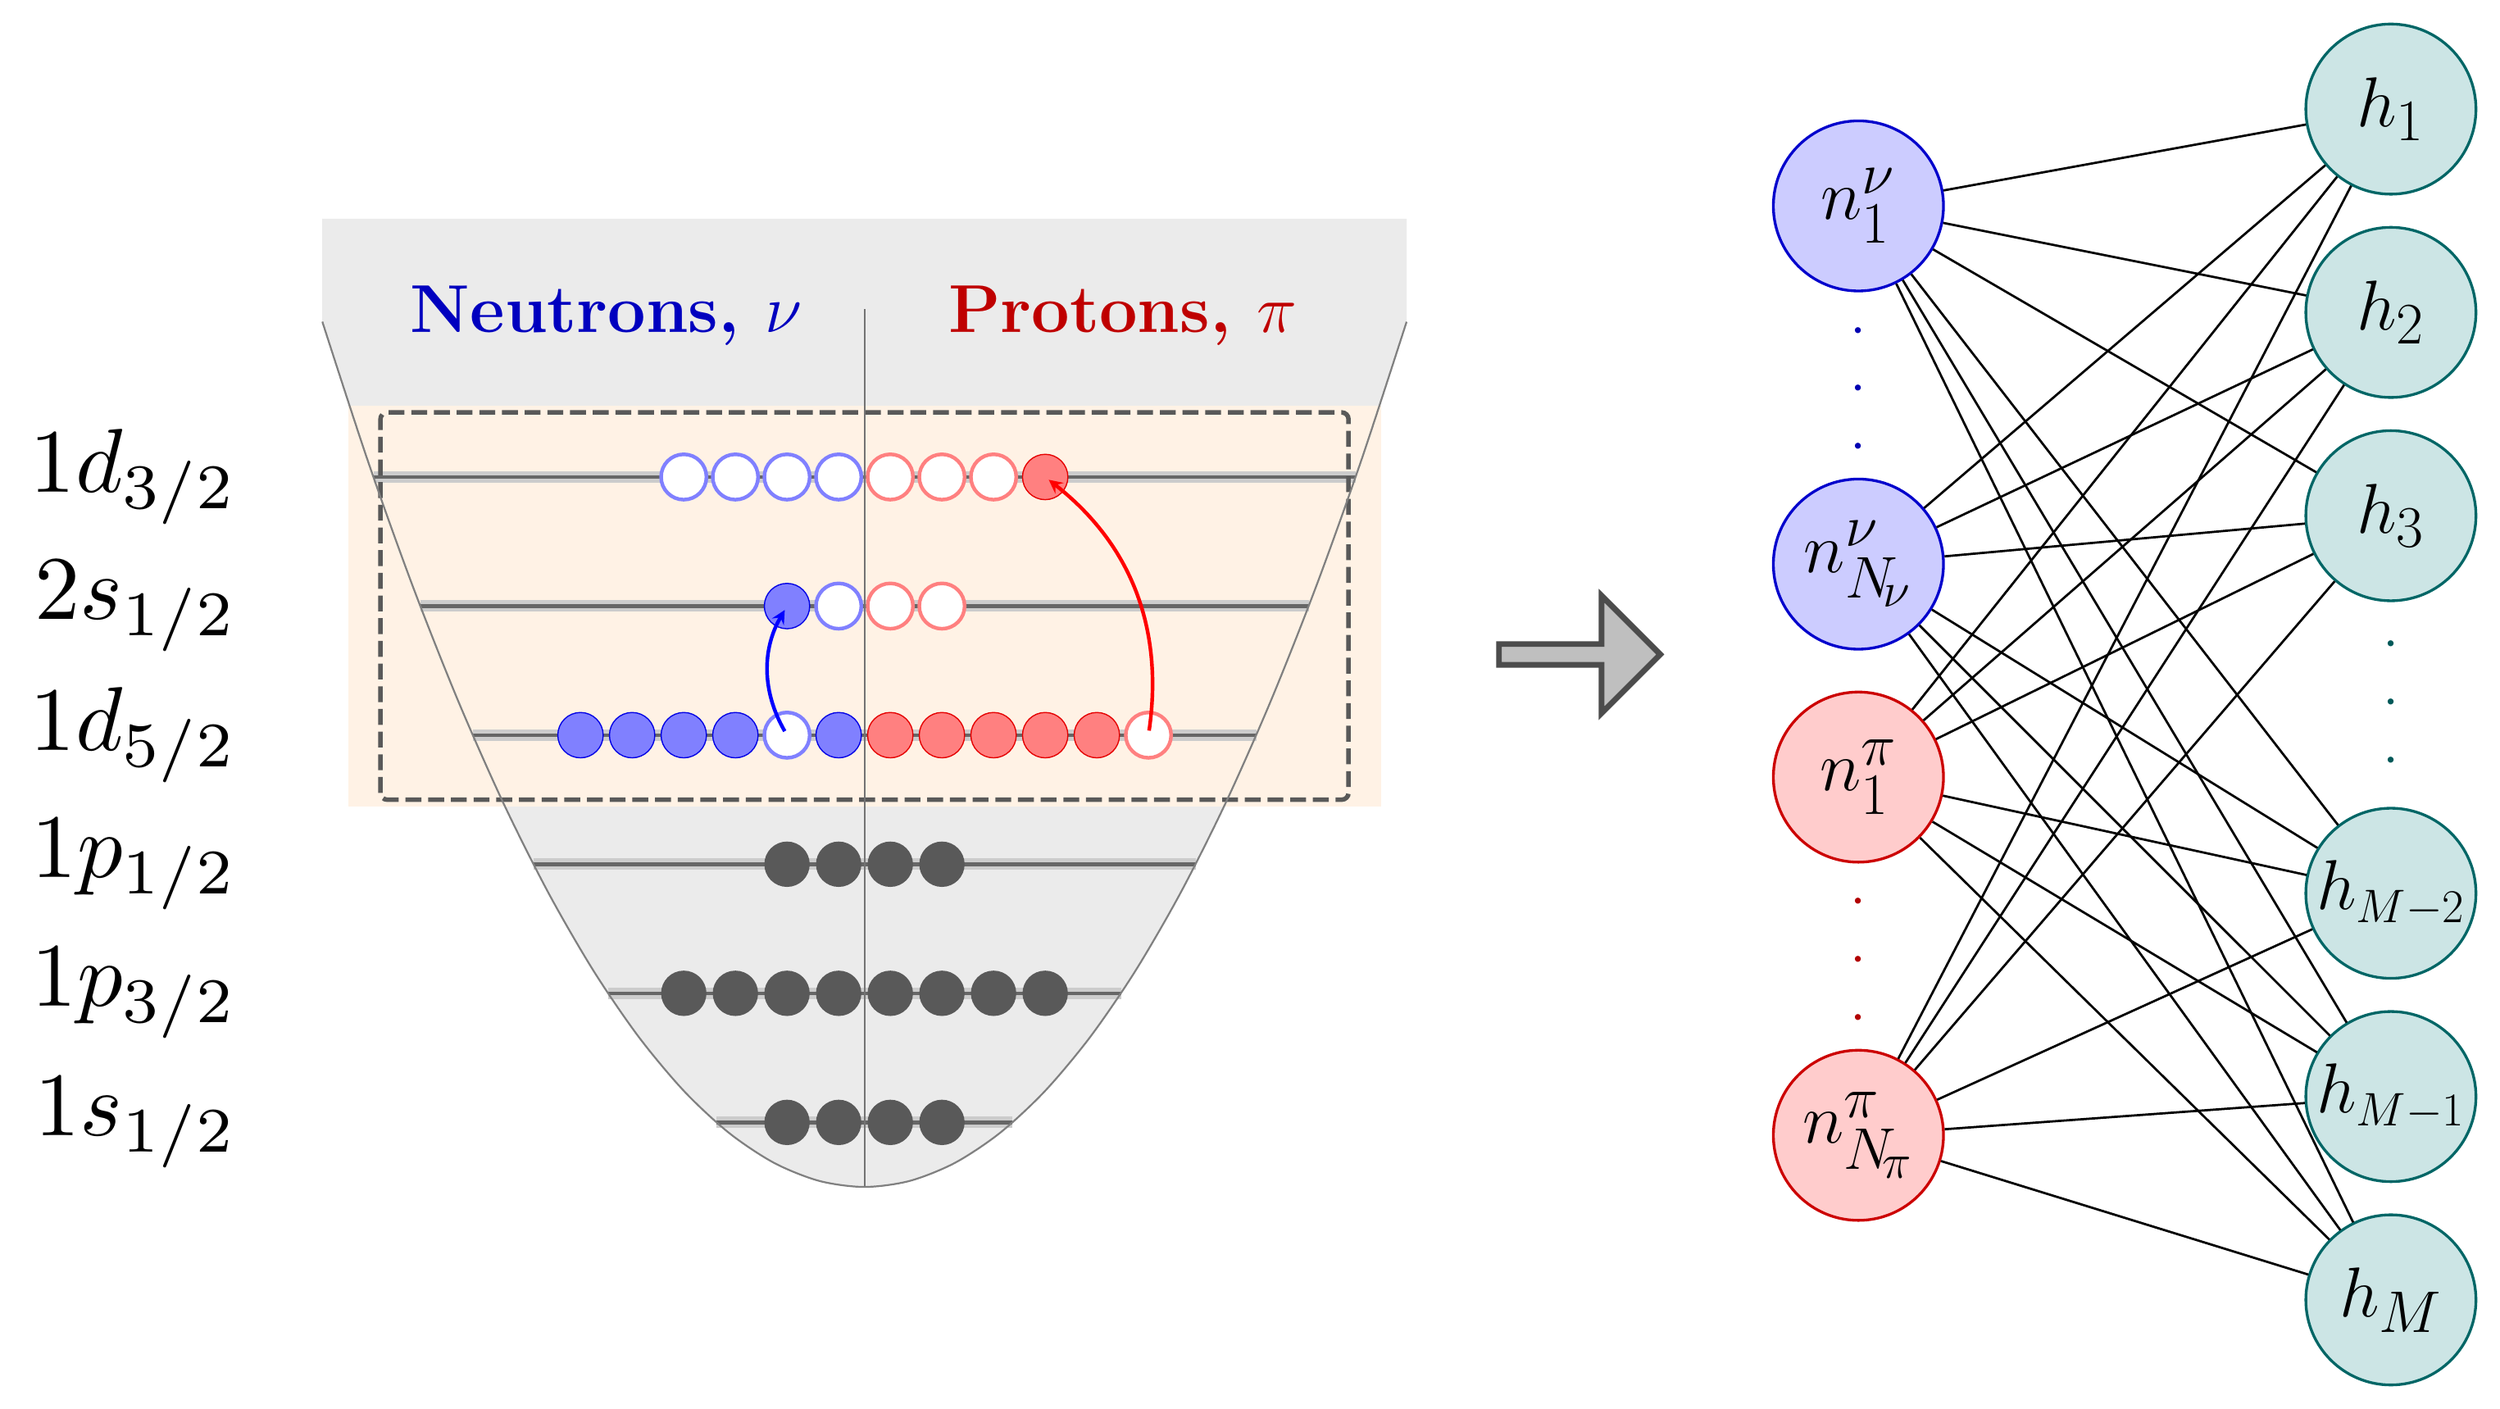
\begin{tikzpicture}[>=stealth]

    \def\labelx{4.8}
    \def\circlesize{5pt}

    \begin{scope}[scale=2, shift={(-6.5, 0)}]

        \fill[black!8, domain=-4.2:4.2, smooth, variable=\x]
            plot ({\x}, {0.38*\x*\x - 5.5}) -- (4.2, 2) -- (-4.2, 2) -- cycle;

        \node[blue!75!black, font=\Huge\bfseries, scale=1.2]
            at (-2., 1.25) {Neutrons, $\nu$};
        \node[red!75!black, font=\Huge\bfseries, scale=1.2]
            at (2., 1.25) {Protons, $\pi$};

        \fill[orange!10] (-4.0,-2.55) rectangle (4.0,0.55);

        \foreach \y/\orblabel/\halfwidth in {
          -5/{$1s_{1/2}$}/1.147,
          -4/{$1p_{3/2}$}/1.987,
          -3/{$1p_{1/2}$}/2.565,
          -2/{$1d_{5/2}$}/3.035,
          -1/{$2s_{1/2}$}/3.441,
           0/{$1d_{3/2}$}/3.804
        } {
          \draw[black!20, line width=5pt]   (-\halfwidth,\y) -- (\halfwidth,\y);
          \draw[black!60, line width=1.6pt] (-\halfwidth,\y) -- (\halfwidth,\y);
          \node[left, black!100] at (-\labelx,\y)
              {\scalebox{4}{\bfseries\itshape\orblabel}};
        }

        \foreach \x in {-0.6, -0.2}
            { \fill[gray!70!black] (\x,-5) circle (\circlesize); }
        \foreach \x in {-1.4, -1.0, -0.6, -0.2}
            { \fill[gray!70!black] (\x,-4) circle (\circlesize); }
        \foreach \x in {-0.6, -0.2}
            { \fill[gray!70!black] (\x,-3) circle (\circlesize); }

        \foreach \x in {-0.6, -0.2}
            { \fill[gray!70!black] (-\x,-5) circle (\circlesize); }
        \foreach \x in {-1.4, -1.0, -0.6, -0.2}
            { \fill[gray!70!black] (-\x,-4) circle (\circlesize); }
        \foreach \x in {-0.6, -0.2}
            { \fill[gray!70!black] (-\x,-3) circle (\circlesize); }

        \foreach \x in {-2.2, -1.8, -1.4, -1.0, -0.2}
            { \fill[blue!50] (\x,-2) circle (\circlesize);
              \draw[blue!90!black, line width=0.5pt] (\x,-2) circle (\circlesize); }

        \fill[white] (-0.6,-2) circle (\circlesize);
        \draw[blue!50, line width=1.6pt] (-0.6,-2) circle (\circlesize);

        \fill[blue!50] (-0.6,-1) circle (\circlesize);
        \draw[blue!90!black, line width=0.5pt] (-0.6,-1) circle (\circlesize);

        \fill[white] (-0.2,-1) circle (\circlesize);
        \draw[blue!50, line width=1.6pt] (-0.2,-1) circle (\circlesize);

        \foreach \x in {-0.2, -0.6, -1.0, -1.4}
            { \fill[white] (\x,0) circle (\circlesize);
              \draw[blue!50, line width=1.6pt] (\x,0) circle (\circlesize); }

        \foreach \x in {-1.8, -1.4, -1.0, -0.6, -0.2}
            { \fill[red!50]  (-\x,-2) circle (\circlesize);
              \draw[red!90!black, line width=0.5pt] (-\x,-2) circle (\circlesize); }

        \fill[white] (2.2,-2) circle (\circlesize);
        \draw[red!50, line width=1.6pt] (2.2,-2) circle (\circlesize);

        \fill[red!50] (1.4,0) circle (\circlesize);
        \draw[red!90!black, line width=0.5pt] (1.4,0) circle (\circlesize);

        \foreach \x in {0.2, 0.6}
            { \fill[white] (\x,-1) circle (\circlesize);
              \draw[red!50, line width=1.6pt] (\x,-1) circle (\circlesize); }

        \foreach \x in {0.2, 0.6, 1.0}
            { \fill[white] (\x,0) circle (\circlesize);
              \draw[red!50, line width=1.6pt] (\x,0) circle (\circlesize); }

        \draw[black!65, line width=0.7mm, rounded corners=3pt,
              dash pattern=on 7pt off 3pt]
            (-3.75,-2.5) rectangle (3.75,0.5);

        \draw[->, blue!100!black, line width=1.6pt, bend left=30,
              shorten >=2pt, shorten <=2pt]
            (-0.6,-2) to (-0.6,-1);
        \draw[->, red!100!black, line width=1.6pt, bend right=30,
              shorten >=2pt, shorten <=2pt]
            (2.2,-2) to (1.4, 0);

        \draw[=>, thick, black!55] (0,-5.5) -- (0,1.3);

        \draw[thick, black!50, domain=-4.2:4.2, smooth, variable=\x]
            plot ({\x}, {0.38*\x*\x - 5.5});

    \end{scope}

    \node[single arrow,
          draw=black!70, fill=black!25,
          minimum height=2.5cm, minimum width=1.8cm,
          single arrow head extend=0.75cm,
          line width=2.5pt]
        at (-2, -2.75) {};

    \begin{scope}[scale=1.2, shift={(2, 3.5)}, x=2.5cm, y=2.5cm]

        \tikzstyle{visible proton}=[
            circle, draw=red!80!black, line width=1.2pt,
            fill=red!20, minimum size=75pt, inner sep=0pt,
            font=\Huge, text=black!90!black]
        \tikzstyle{visible neutron}=[
            circle, draw=blue!80!black, line width=1.2pt,
            fill=blue!20, minimum size=75pt, inner sep=0pt,
            font=\Huge, text=black!90!black]
        \tikzstyle{hidden neuron}=[
            circle, draw=teal!80!black, line width=1.2pt,
            fill=teal!20, text=black!90!black, minimum size=75pt,
            inner sep=0pt, font=\Huge]

        \node[visible neutron] (vnu1) at (0,  0.000) {\scalebox{1.25}{$n^{\nu}_{1}$}};
        \node[font=\Huge, color=blue!70!black] at (0, -0.65) {$\cdot$};
        \node[font=\Huge, color=blue!70!black] at (0, -0.95) {$\cdot$};
        \node[font=\Huge, color=blue!70!black] at (0, -1.25) {$\cdot$};
        \node[visible neutron] (vnuN) at (0, -1.85) {\scalebox{1.25}{$n^{\nu}_{N_{\!\nu}}$}};

        \node[visible proton]  (vpi1) at (0, -2.95) {\scalebox{1.25}{$n^{\pi}_{1}$}};
        \node[font=\Huge, color=red!70!black] at (0, -3.60) {$\cdot$};
        \node[font=\Huge, color=red!70!black] at (0, -3.90) {$\cdot$};
        \node[font=\Huge, color=red!70!black] at (0, -4.20) {$\cdot$};
        \node[visible proton]  (vpiN) at (0, -4.80) {\scalebox{1.25}{$n^{\pi}_{N_{\!\pi}}$}};

        \node[hidden neuron] (h1) at (2.75,  0.50) {\scalebox{1.25}{$h_{1}$}};
        \node[hidden neuron] (h2) at (2.75, -0.55) {\scalebox{1.25}{$h_{2}$}};
        \node[hidden neuron] (h3) at (2.75, -1.60) {\scalebox{1.25}{$h_{3}$}};
        \node[font=\Huge, color=teal!70!black] at (2.75, -2.27) {$\cdot$};
        \node[font=\Huge, color=teal!70!black] at (2.75, -2.57) {$\cdot$};
        \node[font=\Huge, color=teal!70!black] at (2.75, -2.87) {$\cdot$};
        \node[hidden neuron] (h4) at (2.75, -3.55)
        {\scalebox{1.25}{$h$}$_{M-2}$};
        \node[hidden neuron] (h5) at (2.75, -4.60)
        {\scalebox{1.25}{$h$}$_{M-1}$};
        \node[hidden neuron] (hM) at (2.75, -5.65) {\scalebox{1.25}{$h_{M}$}};

        \foreach \vi in {vpi1, vpiN, vnu1, vnuN} {
            \foreach \hj in {h1, h2, h3, h4, h5, hM} {
                \draw[black!100, line width=1pt] (\vi) -- (\hj);
            }
        }

    \end{scope}

\end{tikzpicture}
\end{document}
